%In the first part of this chapter, we give a brief introduction to the \SM~(SM), which forms
%the theoretical basis of the work described in this thesis. The second
%half gives a short introduction into the phenomenology of hadron
%colliders.

\section{The Standard Model}

\todo{This section is copy-pasted from Felix's thesis. Modify heavily the wording.}

The \emph{Standard Model} of particle physics unifies the description of three of the
four known fundamental forces: electromagnetism, weak, and strong.

The SM is a quantum field theory (QFT) on the background Minkowski space-time.
The invariance under translations and rotations in space-time, which make up
the Poincaré group, is built in the theory through as a symmetry of its local
action. Each particle is associated to a field. The transformations properties of
each field determine \emph{spin} of the particles.

The interactions of particles are realized as gauge symmetries.
In particular the SM gauge group is
\begin{align}\label{eq:SMgauge}
  SU(3)_C\times SU(2)_W \times U(1)_Y,
\end{align}
where $SU(2)_W \times U(1)_Y$ describes theory of \emph{electroweak} (EW)
interaction also known as the Glashow-Weinberg-Salam theory \cite{Glashow1961a,Weinberg1967a,Salam1968,Glashow1970},
and $SU(3)_C$ describes the strong force, or \emph{Quantum Chromodynamics} (QCD).


In the following, we describe several aspects of the theory background of the
SM. In particular, we aim at illustrating the concepts of gauge
invariance and spontaneous symmetry breaking. There are many
excellent books on the subject, we partly follow the description in \cite{PeskinS,Schwartz:2013pla}.

\subsection{Gauge Invariance and the Yang-Mills Lagrangian}
\label{sec:giym}
The concept of local gauge symmetry is fundamental to the construction
of the SM Lagrangian. It is based on the assumption, that
certain (continuous) symmetries hold for the physical systems we
describe. Taking the viewpoint that symmetry
is fundamental, one can \textit{derive} the SM Lagrangian\footnote{Historically, the correct gauge group for
  theories only developed over time, with the careful analysis of
  experimental data.}. In the following, we will
illustrate the concept of local gauge invariance for the gauge group
$U(1)$ and see how replacing
the standard derivative with a gauge-covariant derivative assures gauge invariance of kinetic terms in
the Lagrangian. The additional fields introduced in this \textit{minimal
  replacement} are called gauge fields. We will furthermore apply the argument to
non-abelian gauge groups.

%\subsubsection{$U(1)$ gauge invariance and the QED Lagrangian}
\label{sec:qedu1}
\label{sec:ymlagrang}
The case of Quantum Electrodynamics (QED) will serve as a
pedagogical illustration of the concept, since it constitutes a
simple, yet non-trivial application of local gauge invariance. We consider a relativistic QFT with an internal, local $U(1)$ symmetry and
the Lagrangian for free massive fermions, i.e.\ for a complex valued Dirac field
$\psi$, that is given by
\begin{align}
  \mathcal{L}_{\text{Dirac}} = \bar{\psi}(i\slashed{\partial}-m)\psi.\label{eq:diraclag}
\end{align}
Transformations under the internal $U(1)$ group are complex phase
rotations, with a position dependent phase $\alpha(x)$.\footnote{If the
function $\alpha$ is constant, one speaks of a global symmetry.} That is the
symmetry transformations can be different on different points in space-time:
\begin{align}\label{eq:diractrafo}
  \psi(x) &\rightarrow e^{i\alpha(x)}\psi(x),&  \bar{\psi}(x) &\rightarrow e^{-i\alpha(x)}\bar{\psi}(x).
\end{align}
Obviously, the mass term $m\bar{\psi}\psi$ in
the Lagrangian is invariant under this transformation, since the conjugation leads to
the cancellation of the $\alpha$ dependence.

However, as soon as we have terms with derivatives, we cannot naively apply this
transformation and preserve the invariance of $\mathcal{L}$. The directional derivative with respect to a vector
$n^\mu$ is defined as
\begin{align}
    n^\mu \partial_\mu \psi = \lim_{\epsilon \rightarrow 0}
  \frac{1}{\epsilon}\left[\psi(x+\epsilon n)-\psi(x) \right].
\end{align}
It therefore relates the field at points $x$
and $x+\epsilon n$, each of which has a different associated phase
$\alpha(x)$ and $\alpha(x+\epsilon n)$ respectively, which in general breaks the
invariance of $\mathcal{L}$ under the gauge transformation. In the principle of
\textit{minimal replacement}, we replace ordinary derivatives with the covariant derivative 
\begin{align}\label{eq:fincovder}
 D_\mu \psi(x) = \partial_\mu\psi(x)+ieA_\mu\psi(x),
\end{align}
where the gauge field $A^\mu$ transforms as 
\begin{align}\label{eq:photontrafo}
  A_\mu(x) \rightarrow   A_\mu(x) - \frac{1}{e}\partial_\mu \alpha(x).
\end{align}
Using the transformation properties of $A_\mu$ and the field
$\psi(x)$, we can now check that the covariant derivative indeed yields
the desired transformation property
\begin{align}
\begin{split}
 D_\mu \psi(x)\rightarrow \left[\partial_\mu+ie\left(A_\mu-\frac{1}{e}
     \partial_\mu (\alpha)\right) \right]e^{i\alpha(x)} \psi(x)\\
= e^{i\alpha(x)}\left(\partial_\mu + i e A_\mu \right) \psi(x) =
e^{i\alpha(x)}D_\mu \psi(x).
\end{split}
\end{align}
Promoting the partial derivative in Eq.~\eqref{eq:diraclag} to a
covariant derivative, we obtain a kinematic term $\bar{\psi} \slashed{D}
\psi$ that is invariant under local $U(1)$ gauge
transformations. The existence of the photon field $A_\mu$ is thus a
consequence of the principle of local gauge invariance, if one
considers the latter to be fundamental. To complete the construction, we also need a kinematical term for
the photon field $A_\mu$. Instead of deriving it, we check that the known form of the field-strength tensor
is indeed gauge invariant under $U(1)$ transformations
\begin{align}
\begin{split}
  F_{\mu\nu}=\partial_\mu A_\nu - \partial_\nu A_\mu
  \rightarrow&\hspace{0.2cm} \partial_\mu (A_\nu -\frac{1}{e}\partial_\nu \alpha)
  - \partial_\nu (A_\mu-\frac{1}{e}\partial_\mu \alpha) =  F_{\mu\nu}.
%&=F_{\mu\nu} -\frac{1}{e}(\partial_\mu\partial_\nu-\partial_\nu\partial_\mu)\alpha= F_{\mu\nu}.
\end{split}
\end{align}
As an aside, we can observe that $U(1)$ gauge invariance forbids a photon
mass, since the combination $m^2A^\mu A_\mu$ is not gauge
invariant. This problem will resurface later, when the problem of
assigning a mass to gauge bosons of other symmetry groups will
motivate the concept of electroweak symmetry breaking and the introduction of
the Higgs field. 

Imposing the principle of local gauge invariance and the internal
symmetry group $U(1)$ thus leads to the additional vector field
$A_\mu$, which through its coupling to fermions leads to the correct
transformation properties of the Lagrangian. We will now extend this
concept to more general gauge groups, in particular that of $SU(N)$
transformations, which will allow us to construct the Lagrangian of
QCD and later the full SM.

%\subsubsection{Yang-Mills theory and the QCD Lagrangian}
We now aim at generalizing the principle of local gauge invariance
to other continuous internal symmetry groups, in particular to the special
unitary group $SU(N)$ of degree $N$, the group of unitary $N\times N$
matrices with determinant 1. We arrange $N$ fermions into an
$N$-component object 
\begin{align}
  \Psi(x) \equiv (\psi_1,\dots,\psi_N).
\end{align}
The field transformation is thus
given by 
\begin{align}\label{eq:gentrafo}
  \Psi(x) \rightarrow V(x)\Psi(x),
\end{align}
with $V(x)$ being a unitary $N\times N$ dimensional matrix. The
elements $V(x)$
of a Lie group $G$ can be written as $V(x)=\exp(i\alpha^a
  T^a)$, where $T^a$ is a hermitian matrix in the case of $SU(N)$ and we sum over repeated
  indices $a$. Expanding this relation for infinitesimal transformations, we get
\begin{align}
  V(x) = 1 +i\alpha^a(x) T^a +\mathcal{O}(\alpha^2).
\end{align}
The hermitian matrices $T^a$ are the generators of the Lie group. The
associated simple Lie
algebra is defined by the vector space spanned by the generators
as well as the commutator relation between them
\begin{align}\label{eq:commgen}
  [T^a,T^b] = i\sqrt{2}f^{abc}T^c,
\end{align}
for $\Tr(T^aT^b)=1$. The completely anti-symmetric structure constants $f^{abc}$ are a set
of numbers. Symmetries with non-commuting transformations
$V(x)$ ($f^{abc}\neq 0$) are called non-abelian whereas those with commuting
transformations are called abelian ($f^{abc}=0$). We now generalize the covariant derivative, cf.~Eq.~\ref{eq:fincovder},
to $SU(N)$ transformations. Lagrangians that are invariant under $SU(N)$ symmetry
transformations can then be constructed by writing down all possible
terms formed by fields and covariant derivatives thereof. The covariant
derivative associated to the general transformation
\eqref{eq:gentrafo} is a generalization of
Eq.~\eqref{eq:fincovder}
\begin{align}\label{eq:covderym}
  D_\mu = \partial_\mu - i g A^a_\mu T^a.
\end{align}
Each independent generator of the local symmetry thus implies one additional vector
field. The infinitesimal transformation laws for the fields $\Psi(x)$
and $A_\mu^a$ are then analogously given by
\begin{align}
  \Psi(x) \rightarrow & \left(1+i\alpha^a(x)T^a+\mathcal{O}(\alpha^2)\right)\Psi(x), & A_\mu^a\rightarrow & A_\mu^a + \frac{1}{g}\partial_\mu \alpha^a +
f^{abc} A_\mu^b\alpha^c,
\end{align}
where the last term in the transformation of the gauge field $A_\mu^a$
reflects the non-abelian properties of $SU(N)$ and reduces for
$f^{abc}=0$ to the abelian case. From these
infinitesimal transformations, we can deduce the finite
transformations of the gauge field
\begin{align}
   A_\mu^a(x)T^a \rightarrow   V(x)\left[A_\mu^aT^a + \frac{i}{g}\partial_\mu \right]V^\dagger(x).
\end{align}
As for the $U(1)$ symmetry, the transformation properties of $A_\mu^a$ give the
desired transformation properties of the covariant derivative,
i.e.\ the covariant derivative has the same transformation properties
as the field $\Psi$ itself. The field strength tensor for this group is
\begin{align}
  F_{\mu\nu}^a=\partial_\mu A_\nu^a - \partial_\nu A_\mu^a
  +gf^{abc}A_\mu^bA_\nu^c,
\end{align}
where the last term is related to the non-abelian nature of the
gauge group. Note that the field-strength tensor for a non-abelian
theory is no longer a gauge invariant quantity. Expressions containing the field-strength tensor with contracted indices however are gauge and Lorentz invariant and we can construct a so called Yang-Mills
Lagrangian by
\begin{align}\label{eq:ymlag}
  \mathcal{L}_{\text{YM}}=-\frac{1}{4}F^a_{\mu\nu}F^{a\,\mu\nu},
\end{align}
with self-interacting gauge fields that form cubic and quartic terms in the
field. Another important observation is that explicit mass terms are prohibited as
they would violate $SU(N)$ gauge invariance, i.e.\ the pure gauge
bosons are massless.


\subsection{Electroweak Symmetry Breaking and GSW Theory}
\label{sec:gws}
The unified description of weak interactions and electromagnetism in
terms of a gauge theory is more subtle. It is known from experiment that the electroweak force is
mediated by the massive $W^\pm$ and $Z$ vector bosons as well as the
massless photon. In a theoretical description, both the problems of assigning a mass to the gauge fields as well
as respecting perturbative
unitarity bounds in gauge boson scattering were resolved by the
postulation of the Higgs mechanism\footnote{Sometimes referred to as the \textit{Englert-Brout-Higgs-Guralnik-Hagen-Kibble}
  \cite{Guralnik1964,Kibble1967} mechanism of spontaneous symmetry breaking.} in 1964
\cite{Higgs1964b,Higgs1964,Englert1964,Higgs1966}. It is based on
spontaneous symmetry breaking of the combination $SU(2)_W\times U(1)_Y$ of the SM gauge group and introduces an additional scalar field, the
Higgs field. In 2012, both the ATLAS and CMS collaborations at the LHC
succeeded in detecting this last missing and long-predicted ingredient
of the SM, the Higgs boson \cite{hdiscatlas,hdisccms}. The gauge theory of the combined gauge group $SU(2)_W\times
U(1)_Y$ is also referred to as the \ew~sector of the SM. In this subsection, we will briefly illustrate spontaneous
symmetry breaking of a local symmetry and introduce the Higgs mechanism. We partly follow the description in Ref.~\cite{Dittmaier:2012nh}.

\subsubsection{Spontaneous symmetry breaking of a local continuous symmetry - an illustrative example}
\label{sec:spontbreak}
We will briefly present the Abelian Higgs model, where a local $U(1)$
gauge symmetry is spontaneously broken. The starting point is a given Lagrangian invariant under (local) gauge
transformations of some group $G$. Two inequivalent situations exist regarding the ground state
of a system governed by this Lagrangian. Either a unique state of
lowest energy exists and is therefore invariant under group
transformation. Or a set of degenerate, physically equivalent ground
states exists, which transform into themselves under group
transformation of $G$. If one of the states from this set is chosen
as the ground state of the theory,
%\footnote{Spontaneous symmetry  breaking thus only occurs in systems with an infinite number of degrees of freedom, since otherwise the ground state would be an average over all degenerate states due to tunneling.}
the symmetry
$G$ is said to be spontaneously broken. 
%Spontaneous symmetry breaking is known in different areas of physics,
%it is for example used in condensed matter physics to describe a ferromagnetic system
%\footnote{The rotational symmetry of Heisenberg`s spin model does not
%apply to the ground state (all spins up or down). Below the critical
%Curie temperature, the ground state is directed and spontaneously breaks the rotational symmetry.}.

In the Abelian Higgs model, the Lagrangian of a complex scalar field is coupled to both an electromagnetic (gauge) field and itself 
\begin{align}\label{eq:sclag}
  \mathcal{L} = -\frac{1}{4}(F_{\mu\nu})^2+|D_\mu \phi|^2 - V(\phi),
\end{align}
with the covariant derivative $D_\mu = \partial_\mu + i e A_\mu$ and
the square of the modulus denoted by $|\cdot|$. The
Lagrangian is invariant under the transformations $\phi(x) \rightarrow
e^{i\alpha(x)} \phi(x)$ for the scalar field and
\eqref{eq:photontrafo} (for the gauge field $A_\mu$), i.e.\ under local $U(1)$ gauge
transformations. We choose a potential of the form 
\begin{align}\label{eq:scpot}
  V(\phi) = -\mu^2\phi^*\phi+\frac{\lambda}{2}(\phi^*\phi)^2,
\end{align}
with $\lambda >0$, which can develop a
local maximum. The lowest energy configuration of the field $\phi$ depends on the
sign of the parameter $\mu^2$. If $\mu^2<0$, the state of lowest energy is $\phi_0=0$
and the symmetries of the Lagrangian are preserved by the ground state. 
%The theory then corresponds to scalar QED with a massless photon and a charged, self-interacting, complex scalar of mass $\sqrt{|\mu|}$. 
If $\mu^2>0$, the field $\phi_0$ whose value
minimizes the potential is non-zero and fixed by the condition
\begin{align}\label{eq:alphah}
  \phi_{0,\alpha} = \sqrt{\frac{\mu^2}{\lambda}}e^{i\alpha},
\end{align}
with a phase $\alpha$. The field therefore acquires a non-zero vacuum-expectation value
(vev) given by
\begin{align}\label{eq:scalarvev}
  \expval{\phi}\equiv\expval{\phi}{0} = \phi_{0,\alpha} = \sqrt{\frac{\mu^2}{\lambda}}e^{i\alpha}.
\end{align}
The possible ground states are related by $U(1)$ symmetry
transformations. Conversely, choosing one of the states in Eq.~\eqref{eq:scalarvev}
as the vacuum state, the $U(1)$ symmetry is not obeyed anymore, it is said to be spontaneously
broken. If we want to formulate a perturbation theory for $\mu^2>0$,
we have to expand the scalar field around one of the ground states
\eqref{eq:scalarvev} \footnote{The fields corresponding to particles
  are linear in
  creation and annihilation operators and thus have a vanishing vev. Therefore
  only the combination $\psi = \phi-v$ allows for a particle interpretation.}
\begin{align}
  \phi(x) = v + \frac{1}{\sqrt{2}}\left(h(x)+i\chi(x)\right),
\end{align}
and the scalar potential Eq.~\eqref{eq:scpot} then takes the form
\begin{align}
  V(\phi) =  -\frac{1}{2\lambda}\mu^4+\frac{1}{2}2\mu^2h^2+\textit{(cubic
  and quartic terms)}.
\end{align}
The real field $h$ is referred to as the Higgs boson and acquires a
mass $m=\sqrt{2}\mu$ and the massless real field
$\chi$ is referred to as would-be Goldstone boson
\cite{Goldstone1961,Goldstone1962}, since the field would correspond to a Goldstone boson in an ungauged theory. We use the above
expansion around the vev and obtain for the kinematic term of $\phi$ in Eq.~\eqref{eq:sclag}
\begin{align}
  |D_\mu \phi|^2 = \sum_{i=1}^2\frac{1}{2}\left(\partial_\mu\phi_i\right)^2+\sqrt{2}ev
  A_\mu\partial^\mu\chi+e^2v^2 A_\mu A^\mu+\textit{(cubic
  and quartic terms)}.
\end{align}
Interestingly, the
gauge field $A_\mu$ now has acquired a mass term
\begin{align}
  \mathcal{L} = \frac{1}{2}m_A^2 A^\mu A_\mu,
\end{align}
with a mass $m_A^2=2e^2v^2$ related to the vev of the scalar
field. The interaction between $A^\mu$ and $\chi$ can be removed by a gauge transformation
\begin{align}
  A_\mu(x) \rightarrow A_{\mu}^{\prime} = A_\mu-\frac{1}{\sqrt{2}ev}\partial_\mu \chi,
\end{align}
and the degree of freedom (\dof) of the would-be Goldstone boson delivers the
longitudinal polarization of the now massive gauge field. It becomes clear that such a transformation can always be
found when considering the \dof{} before and after
spontaneous symmetry breaking. We started out with four \dof{}, since the massless gauge boson and complex
scalar field contribute two \dof{}~each. After spontaneous symmetry
breaking, the massive gauge boson has three \dof~and the real scalar
field $h$ one, adding up to four \dof. 

The gauge field $A_\mu$
thus acquires its mass through the
interaction with the vacuum expectation value $v$ after
spontaneous symmetry breaking. The scalar would-be Goldstone boson associated to the
spontaneous symmetry breaking of a local gauge symmetry delivers the
\dof~of the longitudinal polarization of the massive gauge boson. This mechanism is referred to as Higgs
mechanism \cite{Higgs1964b,Higgs1964,Englert1964,Higgs1966}. We will now move away from the illustrative example of the
Abelian Higgs model and additionally require that the spectrum of gauge boson masses
matches the one realized in nature.

\subsubsection{The Gauge Part of Glashow-Weinberg-Salam Theory}
\label{sec:gwsgauge}
In order to reproduce the known spectrum of gauge bosons masses one requires the spontaneous breaking of a non-abelian gauge symmetry. In fact it was the insight of Glashow, Weinberg
and Salam \cite{Glashow1961a,Weinberg1967a,Salam1968,Glashow1970} to
break the combined symmetry of $SU(2)_W\times U(1)_Y$, which then leads to
three massive gauge bosons ($W^\pm,Z$) compatible with the nowadays known mass spectrum and a
residual $U(1)_{em}$ symmetry. The latter naturally describes
electrodynamics with its massless gauge boson, the photon. We first describe the gauge part
of the unified \ew~gauge theory, this is in analogy to
Sec.~\ref{sec:giym}.


The covariant derivative is given by
%\footnote{Note that there are different conventions regarding the
%sign of the terms in the covariant derivative, here we use the convention by B\"ohm \cite{Bohm1986}}
\begin{align}\label{eq:codesu2}
    D_\mu = \partial_\mu + i g_2 I^a_W W^a_\mu + i g_1 \frac{Y_W}{2}B_\mu,
\end{align}
where we have introduced two independent couplings $g_1$ and
$g_2$, since we have two independent gauge groups $SU(2)_W$ and $U(1)_Y$. The generators of $SU(2)_W$
describing weak isospin are called $I_W^a$ and can be represented in
$2$-dimensions by the Pauli matrices $I_W^a=\sigma^a/2$, the $U(1)_Y$ generator $\frac{Y_W}{2}$
is a real number called weak hypercharge. There are three massless
gauge fields $W^a_\mu$ associated to the isospin generators and one
massless gauge field $B_\mu$ associated to the hypercharge
generator. The gauge part of the Lagrangian then obtains kinematic
terms for all four gauge fields and is given by
\begin{align}\label{eq:ewgaugelag}
  \mathcal{L}_{\text{gauge}}=-\frac{1}{4}W^a_{\mu\nu}W^{a,\mu\nu}-\frac{1}{4}B_{\mu\nu}B^{\mu\nu},
\end{align} 
where the index $a$ runs over the associated three generators $I_W^a$.
\subsubsection{The Higgs Mechanism and $W$- and $Z$-boson masses}
\label{sec:gwshiggs}
We now describe how the Higgs mechanism reconciles the experimental fact of
non-vanishing $W$- and $Z$-boson masses with the massless gauge fields
obtained from the unbroken gauge theory. We take the structure from
above, i.e~a $SU(2)_W\times U(1)_Y$ gauge group and the associated
gauge fields, together
with a scalar field $\Phi$ transforming as an $SU(2)$ doublet
\begin{align}
  \Phi = \pmqty{\phi^+ \\ \phi^0},
\end{align}
 with weak hypercharge $Y_W=+1$. In total,
the scalar field $\Phi$ has four \dof. The gauge
transformation of $\Phi$ then becomes
\begin{align}
\Phi \rightarrow e^{i\alpha(x)^a I^a_W}e^{i\beta(x)/2}\Phi.  
\end{align}
The Higgs Lagrangian is given by
\begin{align}\label{eq:higgslag}
  \mathcal{L}_{\text{Higgs}} &= (D_\mu \Phi)^\dagger(D^\mu
  \Phi)-V(\Phi), & V(\Phi)&=-\mu^2(\Phi^\dagger\Phi)+\frac{\lambda}{4}(\Phi^\dagger\Phi)^2,
\end{align}
such that the field $\Phi$ can acquire a non-vanishing vacuum
expectation value for positive $\lambda$ if $\mu^2>0$, determined by
the condition
\begin{align}
  (\Phi^\dagger_0\Phi_0^{\phantom{\dagger}})&=\frac{2\mu^2}{\lambda}\equiv
  \frac{v^2}{2},& v&=2\sqrt{\frac{\mu^2}{\lambda}}.
\end{align}
The vacuum
state is fixed up to a $U(2)$ rotation and conventionally the state 
\begin{align}
\expval{\Phi}\equiv\expval{\Phi}{0}=\Phi_0 = \pmqty{0\\\frac{v}{\sqrt{2}}},
\end{align}
is chosen from the degenerate set of vacuum states. Only gauge transformations of $\Phi$ with $\alpha^1 = \alpha^2 =0$ and
$\alpha_3=\beta$ leave the vacuum state invariant, since the only
combination of generators that annihilates the vacuum is given by
\begin{align}\label{eq:gmnrel}
   \left(I^3_W+\frac{Y_W}{2}\right)\expval{\Phi} = \left(\frac{\sigma^3}{2}+\frac{1}{2}\right) \pmqty{0\\\frac{v}{\sqrt{2}}}=0.
\end{align}
 The
Gell-Mann-Nishijima formula identifies this combination with the
electric charge operator
\begin{align}\label{eq:GMN}
  Q\equiv I^3_W+\frac{Y_W}{2},
\end{align}
and it becomes clear that $\phi^+$ carries charge
 $+e$ and $\phi^0$ is neutral. 
%The vanishing of the upper component of $\Phi_0$ thus reflect the requirement that the vev is neutral.
Gauge transformations with the charge operator $Q$ leave the vacuum state invariant
\begin{align}
   e^{iQ}\expval{\Phi} =( 1 + Q + \cdots)\expval{\Phi} = \expval{\Phi},
\end{align}
where we used Eq.~\eqref{eq:gmnrel}. The gauge group $SU(2)_{W}\times
U(1)_Y$ is thus broken in such a way, that it still contains one
unbroken $U(1)_{\text{em}}$ symmetry with the associated massless gauge field corresponding to the photon.


As in the abelian Higgs model, we expand the scalar field $\Phi$ around the vacuum expectation
value, such that we get fields with vanishing vev
\begin{align}\label{eq:scaexp}
\Phi=\pmqty{\phi^+\\\frac{1}{\sqrt{2}}\left(v+H(x)+i\chi(x)\right)},
\end{align}
where the real field $H(x)$ corresponds to the massive physical Higgs
boson and the fields $\phi^+(x)$ and $\chi(x)$, which are complex and
real fields respectively, correspond to would-be Goldstone bosons. The three \dof~of the
would-be Goldstone bosons are unphysical and can be transformed away in an appropriate
gauge, c.f.\ discussion in the previous section on the
Abelian Higgs model. To identify the physical gauge boson masses, we apply a transformation
of the fields into mass and electric charge eigenstates, called
$W^\pm$, $Z$ and $A$, which are related to $W^a$ and $B$ through
\begin{align}\label{eq:chmaeig}
  \pmqty{Z_\mu\\A_\mu}=\pmqty{c_W & -
    s_W\\s_W & c_W}\pmqty{W_\mu^3\\B_\mu}, && W_\mu^{\pm} =
  \frac{1}{\sqrt{2}}(W_\mu^1\mp i W_\mu^2),
\end{align}
with the weak mixing angle $\theta_W$ defined by
\begin{align}
  \cos\theta_W &\equiv c_W=\frac{g_2}{\sqrt{g_1^2+g_2^2}}, &   \sin\theta_W
  &=\sqrt{1-c_W^2}=\frac{g_1}{\sqrt{g_1^2+g_2^2}}.
\end{align}
Both linear combination $W^\pm$ are mass degenerate eigenstates of
$U(1)_{\text{em}}$, i.e.\ $QW_\mu^\pm= I^3_W W_\mu^\pm = \pm
W^\pm_\mu$. We then use Eq.~\eqref{eq:scaexp} in the gauge where the would-be Goldstone bosons are transformed away and insert it into the Higgs
Lagrangian Eq.~\eqref{eq:higgslag}. We can identify mass and
charge eigenstates of Eq.~\eqref{eq:chmaeig} and get the following
Higgs Lagrangian
\begin{align}\label{eq:higgslagmass}
    \mathcal{L}_{\text{Higgs}} =\frac{1}{2}(\partial_\mu
    H)^2+ \left(\frac{g_2^2}{4}W^+_\mu W^{-\,\mu}+
      \frac{g_2^2}{8c_W^2}Z_\mu Z^{\mu}+\frac{\mu^2}{2}
      -\frac{\lambda}{16}(v+H)^2 \right) (v+H)^2.
\end{align}
The terms bilinear in the fields $W^\pm$, $Z$ and $H$ correspond to
mass terms of the corresponding bosons with masses $M_W$, $M_Z$ and
$M_H$, which we can identify in Eq.~\eqref{eq:higgslagmass} as
\begin{align}
  M_W &= \frac{vg_2}{2}, & M_Z &=\frac{ vg_2}{2c_W}=\frac{M_W}{c_W}, &M_H
  &=\sqrt{2\mu^2}, & M_A&=0.
\end{align}
Thus, as in the previous example of the abelian Higgs model, the gauge
fields acquire their mass through an interaction with the scalar
field $\Phi$ after symmetry breaking. The field $H$ corresponds to a
neutral spin-0 particle of mass $M_H$. The Lagrangian in
Eq.~\eqref{eq:higgslagmass} allows for both three- and four-point
interactions of the Higgs boson with a massive weak gauge boson $V=W,Z$. The
$HVV^\dagger$ interactions are proportional to $M_V^2/v$ and
$HHVV^\dagger$ interactions are proportional to $M_V^2/v^2$, as can be
seen from the factor $v^2(1+H/v)^2$ multiplying the gauge boson mass
terms. Furthermore, the Higgs fields is self-interacting with three-
and four-point interactions proportional to $M_H^2$. Before
spontaneous symmetry breaking, we had four massless gauge bosons (8
\dof) and a complex scalar doublet
field $\Phi$ (4 \dof), thus in total twelve \dof. After spontaneous symmetry
breaking, we are left with three massive gauge boson (9 \dof), one
massless gauge boson (2 \dof), and the real Higgs field (1 \dof), which adds up to twelve \dof~as it should.


In summary, we have seen how the spontaneous breaking of the unified
gauge group $SU(2)_W\times U(1)_Y$ for the \ew~sector of the SM
generated a vector boson spectrum that matches the observed
one. Note, that this does not imply a
  prediction about the size of the mass, since it is given in terms of
  \textit{a priori} unconstrained coupling parameters. To spontaneously break the symmetry, we had to introduce an
additional scalar field. Expanding this field around its non-vanishing
vacuum expectation value, we obtained the massive scalar Higgs field. 

\subsection{Matter Content of the Standard Model}
\label{sec:mattercont}
We now discuss how the \ew~gauge bosons couple to fermions and how the
latter acquire their mass in the SM. The fermionic part or matter
content of the SM consists of
leptons ($e,\nu_e,\mu,\nu_\mu,\tau,\nu_\tau$) and quarks
($d,u,s,c,b,t$). The leptons are subject to electromagnetic and weak
interactions and the quarks additionally interact
strongly\footnote{We will suppress the color charge index from
  $SU(3)_C$ in this section for
clarity.}. Each fermion type comes in three generations. The
gauge transformation properties inside a generation are identical but
both mass and flavor differ in generations. The weak force is of chiral nature,
i.e.\ it couples
differently to particles depending on their chirality. With no compelling explanation of why this is the case,
we proceed by describing how the SM accounts for it\footnote{Why the weak force is
  chiral in nature and why
  there are three generations of fermions remain outstandinging problems in physics, an argument for the latter is presented in Ref.~\cite{vanderBij:2007fe}.}.


 Left- and right-handed spin-$\frac{1}{2}$ particles are defined via the
 chirality projector 
 \begin{align}
 \text{P}_{\text{L/R}}&=(1\mp \gamma_5)/2,& \Psi^{\text{L/R}}\equiv  \text{P}_{\text{L/R}} \Psi,
 \end{align}
with the matrix $\g5=i\gamma^0\gamma^1\gamma^2\gamma^3$. Left-handed fermions (leptons $L$ and quarks $Q$) are grouped into pairs, weak
isospin doublets, that transform under $SU(2)_W$ in the
fundamental representation
\begin{align}
 \Psi_{lepton,i}^L \equiv L_i^L\equiv \pmqty{\nu_{i,L}\\l_{i,L}}, && \Psi_{quark,i}^L\equiv Q_i^L \equiv \pmqty{u_{i,L}\\d_{i,L}},
\end{align}
where the index $i$ is running over the three generations and the
particles ($\nu, l$) represent neutrinos and charged leptons
respectively and ($u, d$) represent up- and down-type
quarks. The residual symmetry generators of $SU(2)_W\times
U(1)_Y$ are given by $Q = I_W^3+\frac{Y_W}{2}$, see
Eq.~\eqref{eq:GMN}. Given the associated charge $I_W^3=+\frac{1}{2}$ for
$\nu_{i,L},u_{i,L}$ and $I_W^3=-\frac{1}{2}$ for $l_{i,L},d_{i,L}$ respectively, the weak hypercharge $Y_W$ is fixed such
that the known electric charge values are recovered. Table
\ref{tab:smmatter} gives an overview of
the SM matter fields and their charge assignments. Right-handed particles are uncharged under the weak interaction, i.e.\ are $SU(2)_W$ singlets. We thus have isospin singlets 
\begin{align}
  \Psi_{l,i}^R\equiv l_{i,R}, &&
   \Psi_{u,i}^R\equiv u_{i,R}, &&\Psi_{d,i}^R\equiv d_{i,R},
\end{align}
where the index $i$ is again running over generations. Right-handed
neutrinos are not charged under the SM
gauge group and therefore do not interact with the SM gauge
interactions. We stick to the original formulation of the SM in which right-handed
neutrinos are omitted. 


%%%%%%%%%%%%%%%%%%%%%%%%%%%%%%%%%%%%%%%%
%%%%%%%%%%%%%%%%%%%%%%%%%%%%%%%%%%%%%%%%
%Table SM particles
\begingroup
\renewcommand*{\arraystretch}{1.2}
\begin{table}[]
\centering
\begin{tabular}{llccccrrrr}
\toprule
                        &                              &  \multicolumn{3}{c}{generation} &  rep.   & \multicolumn{3}{c}{charges} \\ \cline{7-9}  \cline{3-5}
                        &                              &   1\textsuperscript{st}    &   2\textsuperscript{nd}    &   3\textsuperscript{rd}   &  &   $I^3_W$    &   $Y_W$    &  $Q$    \\ \hline\\[-13pt]
\multirow{4}{*}{quarks} & \multirow{2}{*}{L}
&\multirow{2}{*}{$\pmqty{u\\d}_L$}&\multirow{2}{*}{$\pmqty{c\\s}_L$}&\multirow{2}{*}{$\pmqty{t\\b}_L$}&
\multirow{2}{*}{($\textbf{3}$,$\textbf{2}$)}  &$\frac{1}{2}$ &$\frac{1}{3}$ &$\frac{2}{3}$\\
                        &                              &       &       &      &  &  $-\frac{1}{2}$    & $\frac{1}{3}$&  $-\frac{1}{3}$    \\
                        & \multirow{2}{*}{R}&  $u_R$     &
                        $c_R$ &$t_R$      &($\textbf{3}$,$\textbf{1}$)& $0$    & $\frac{4}{3}$&  $\frac{2}{3}$    \\
                        &                              &  $d_R$     & $s_R$ &$b_R$      &($\textbf{3}$,$\textbf{1}$)&  $0$     &$-\frac{2}{3}$&  $-\frac{1}{3}$    \\ [1pt] \cline{1-9} \\[-13pt]
\multirow{4}{*}{leptons}& \multirow{2}{*}{L}
&\multirow{2}{*}{$\pmqty{\nu_{e}\\e}_L$}&\multirow{2}{*}{$\pmqty{\nu_{\mu}\\\mu}_L$}&\multirow{2}{*}{$\pmqty{\nu_{\tau}\\
    \tau}_L$}&\multirow{2}{*}{($\textbf{1}$,$\textbf{2}$)}&$\frac{1}{2}$&$-1$&$0$\\
                        &                              &       &       &      && $-\frac{1}{2}$&$-1$ &   $-1$   \\
                        &R& $e_R$      &  $\mu_R$      &    $\tau_R$  &($\textbf{1}$,$\textbf{1}$)&$0$ &$-2$ & $-1$     \\
\bottomrule
\end{tabular}
\caption{Overview of the fermionic matter content of the SM. We show the three generations of quarks
  and leptons of different chirality ($L,R$). The representation in which the corresponding fields transform under the
  SM gauge group is shown in the format ($SU(3)_C,SU(2)_W$). All fields transform as singlets under $U(1)_Y$. The \ew~charges $I_W^3,Y_W$ and $Q$ are specified in the last four
  columns. Table is adapted from \cite{Huss:2014eea}.}
\label{tab:smmatter}
\end{table}
\endgroup
%%%%%%%%%%%%%%%%%%%%%%%%%%%%%%%%%%%%%%%%
%%%%%%%%%%%%%%%%%%%%%%%%%%%%%%%%%%%%%%%%
With the gauge transformation properties of the fermions established,
we can now build the kinetic terms of the fermions in the
Lagrangian. We promote the normal derivative in the free Dirac theory of
massless fermions to the covariant derivative
Eq.~\eqref{eq:codesu2} and obtain
\begin{align}\label{eq:fermlag}
  \mathcal{L}_{\text{Fermion}} = \sum_{i=1}^3\left( \bar{L}_i^L
    \slashed{D}L_i^L + \bar{Q}_i^L \slashed{D}Q_i^L + \bar{l}_i^R
    \slashed{D}l_i^R + \bar{u}_i^R \slashed{D}u_i^R + \bar{d}_i^R \slashed{D}d_i^R \right),
\end{align}
where we again suppress the color indices. 

\subsubsection{Fermion Masses}
\label{sec:fermmass}
Direct and indirect observations show that all fermions are
massive.\footnote{We work with
the approximation of three massless neutrinos. However, the existence of three
  light neutrinos with distinct masses smaller $1$ eV is implied by
  the experimentally well established mixing of three neutrino states.} However, an explicit
formulation of mass terms such as Dirac mass terms $m \left(\bar{\Psi}^R
  \Psi^L + \bar{\Psi}^L
  \Psi^R \right)$ in the Lagrangian violates $SU(2)$ gauge
invariance. They would mix the two chiralities of the fermion
field which transform in different representations of $SU(2)$. Fermion masses can be consistently introduced through an indirect mechanism as in the
case of \ew~gauge boson. Mass terms are generated by an
interaction with the Higgs field, i.e.\ they are dynamically created
and appear only after symmetry breaking. We mention that we work with
the approximation of three massless neutrinos.


With the Higgs field introduced above, the most general gauge
invariant Lagrangian contains a Yukawa coupling \footnote{A Yukawa
  coupling is an interaction between a scalar field and a Dirac
  field of the type $g\bar{\Psi}\phi\Psi$.} between the Higgs
doublet and the chiral fermion fields for leptons and quarks, that is 
\begin{align}\label{eq:yuklag}
  \mathcal{L_{\text{Yukawa}}} = - \sum_{i,j = 1}^3\left(\bar{L}_{i}^L
    G_{ij}^ll^{R}_j\Phi +\bar{Q}_{i}^L G_{ij}^uu_{j}^R\tilde \Phi
    +\bar{Q}_{i}^L G_{ij}^dd_{j}^R\Phi +\text{h.c.}\right),
\end{align}
where the field $\tilde \Phi = (\phi^{0*},-\phi^-)^T$ is the charge conjugate of
the scalar field $\Phi$, with $\phi^-=(\phi^+)^*$. The field $\tilde
\Phi$ transforms under the fundamental representation of $SU(2)$ with
hypercharge~$Y_W=-1$. Note that all terms in
$\mathcal{L_{\text{Yukawa}}}$ are invariant under transformations of
the SM gauge group Eq.~\eqref{eq:SMgauge}. The Yukawa interaction
matrices $G_{ij}^f$ ($f=l,u,d$) are
$3\times 3$ matrices in generation space. The fields written above are
in the flavor basis of left- and right-handed fields, therefore the Yukawa
matrices do not have to be diagonal. The non-diagonal elements of
$G_{ij}^f$ mix fermions of type $f$ from different generations. Since the fields $\Phi$ and $\tilde \Phi$ contain a constant piece
proportional to the vev $v$, $\mathcal{L_{\text{Yukawa}}}$ contains
mass terms for the fermion fields. A diagonalization of the matrices
$G^f_{ij}$ is achieved by the unitary transformations
\begin{align}\label{eq:trafomb}
  \hat{f}_i^{L}=\sum_{j = 1}^3U_{ij}^{f,L}f_j^{L},&&  \hat{f}_i^{R}=\sum_{j = 1}^3U_{ij}^{f,R}f_j^{R},
\end{align}
where $f$ denotes the fermion type $f=l, u, d$. The mass terms of
the fermion fields in the new mass basis (denoted by a hat) become
transparent and are related to the Higgs vev
\begin{align}\label{eq:diagyuk}
 U^{f,L}G^{f}\left(U^{{f},R}\right)^\dagger =
 \frac{\sqrt{2}}{v} \pmqty{m_{f^\prime,1} &0&0\\0&m_{f^\prime,2}&0\\0&0&m_{f^\prime,3} }, 
\end{align}
with fermion masses $m_{f,i}$. The Yukawa part of the Lagrangian thus takes on the simple form
\begin{align}
    \mathcal{L_{\text{Yukawa}}} = - \sum_{f,i}m_{f,i}\left(\bar{f}^L_i f^R_i
      +\bar{f}^R_i f^{L}_i\right)\left(1+\frac{H}{v}\right),
\end{align}
with the summation running over the three generations $i$ and fermion
types $f=l,u,d$ and the gauge in which the would-be Goldstone bosons are absent is used. The Yukawa coupling between fermions and the Higgs
field is thus proportional to $m_{f,i}/v$. The field redefinitions of
Eq.~\eqref{eq:trafomb} have several effects on the SM
Lagrangian. Fermion fields are replaced by those in the mass basis
(and the hat notation is conventionally dropped),
the Yukawa coupling matrices are replaced with their diagonal form
Eq.~\eqref{eq:diagyuk} and charged-current interactions receive a
modification from the matrices $U$, whereas neutral current
interactions remain unchanged since they do not mix up- and down-type quarks. The interaction of $W^{1}$ and $W^2$
with quarks via the
covariant derivative Eq.~\eqref{eq:codesu2} was given in
\eqref{eq:fermlag}. Since $\sigma^1$ and $\sigma^2$ are off-diagonal,
$W^{1}$ and $W^2$ do connect $u$- and $d$-type
quarks of one generation. The transformations in
Eq.~\eqref{eq:trafomb} now imprint a non-diagonal mixing across generations in the $W$-coupling
matrix. The matrix parameterizing this mixing is called the
Cabbibo-Kobayashi-Maskawa \cite{Cabibbo1963,Kobayashi1973} (CKM)
matrix\footnote{In the approximation of three massless neutrinos, the left-handed neutrino fields are transformed by the same unitary matrix as their charged counterparts and the analogous neutrino mixing matrix, called Pontecorvo-Maki-Nakagawa-Sakata (PMNS) matrix, can be transformed away by field redefinitions.} and connected to the mass eigenstate transformation by
\begin{align}
  V_{\text{CKM}} \equiv U^{u,L}\left(U^{d,L}\right)^{\dagger}.
\end{align}

In summary, we have seen some of the underlying concepts of the
SM. In particular, we saw how Lagrangians are constructed out of the SM gauge
group and how masses for both \ew~gauge bosons as well as fermions are generated via the Higgs interactions and spontaneous symmetry
breaking. We can now collect all the pieces that make up the SM Lagrangian\footnote{We suppress CP violating terms of gauge fields such as the $\theta_{FF}$ term.} and obtain by using
Eqs.~\eqref{eq:qcdlag},\eqref{eq:ewgaugelag},\eqref{eq:higgslag},\eqref{eq:fermlag}
and \eqref{eq:yuklag}
\begin{align}
\begin{split}
  \mathcal{L}_{\text{SM}}&=\mathcal{L}_{\text{QCD}}+\mathcal{L}_{\text{EW}}\\
&=\mathcal{L}_{\text{QCD}}+\mathcal{L}_{\text{gauge}}+\mathcal{L}_{\text{Higgs}}+\mathcal{L}_{\text{Fermion,EW}}+\mathcal{L}_{\text{Yukawa}}.
\end{split}
\end{align}



\subsection{Quantization and Gauge Fixing}
\label{sec:quant-gauge-fixing}
We briefly illustrate the concept of quantization and the associated
gauge fixing in the case of QCD. For the more involved case of
\ew~theory, we refer to the literature e.g.\ \cite{Bohm:2001yx}. If we
perform the quantization by following the path-integral formulation,
all gauge field configurations are considered
\begin{align}
  \int \mathcal{D}A_\mu^a\exp{i\int d^4x \mathcal{L}_{\text{YM}}},
\end{align}
including those related by gauge transformations. In order to avoid
the overcounting of physically identical configurations that are
gauge-equivalent, we pick out a specific one which is achieved by
adding a gauge fixing term to the Lagrangian
\begin{align}
  \mathcal{L}_{\text{fix}} = \frac{1}{2\xi}(\partial^\mu A_\mu^a)(\partial^\nu A_\nu^a),
\end{align}
as well as the Faddeev-Popov term
\begin{align}
  \mathcal{L}_{\text{ghost}} = -\bar{c}^\alpha\partial^\mu D_\mu^{\alpha\beta}c^{\beta},
\end{align}
with the covariant derivative in the adjoint representation
$D_\mu^{\alpha\beta}$, $\alpha,\beta=1,\ldots,8$. The ghosts from the
Faddeev-Popov Lagrangian contribute to loop amplitudes. In an
application of the unitarity method, where at least one loop momentum
is forced on the physical mass-shell, unphysical degrees of freedom directly cancel against the ghosts and explicit gauge fixing can be omitted when working with physical polarization states in the loop. Therefore, we omit ghost fields for the rest of this thesis.

\subsection{QCD}
The theory based on the $SU(3)_C$ part of the SM gauge group is called
Quantum Chromodynamics (QCD). It describes the strong force that is
responsible for the binding of quarks into hadronic particles. For the
purpose of this subsection, we treat QCD interaction independent from \ew~interactions. One can combine \ew~theory and QCD by adding up
the non-overlapping Lagrangian terms. Quarks transform
under $SU(3)$ in the three-dimensional fundamental representation
(\textbf{3}) and are thus represented as color triplets
\begin{align}
  q = \pmqty{q_r\\q_g\\q_b},
\end{align}
with the customary assignment of the colors red ($r$), green ($g$) and blue ($b$). The QCD Lagrangian
is build from Eq.~\eqref{eq:diraclag} for the quark field as well as
Eq.~\eqref{eq:ymlag} and reads
\begin{align}\label{eq:qcdlag}
  \mathcal{L}_{\text{QCD}} = -\frac{1}{4}F^a_{\mu\nu}F^{a,\mu\nu} + \sum_f
  \bar{q}_f (i \slashed{D}  -m_f) q_f ,
\end{align}
where the summation runs over all quark flavors $f$ (see Sec.~\ref{sec:mattercont}), the covariant derivative for $SU(3)$ is given in Eq.~\eqref{eq:covderym} and contractions with the four-dimensional
Dirac matrices are denoted as $\slashed{D} \equiv D_\mu \gamma^\mu$. The eight generators of the fundamental
representation of $SU(3)$ can be written in terms of the Gell-Mann
matrices $T^a = \frac{\lambda^a}{\sqrt{2}}$ (explicit expressions can e.g.\ be
found in \cite{Schwartz:2013pla}) and the associated
self-interacting gauge fields are called gluons. 

\subsubsection{Running coupling}
\label{sec:runcoup}

The QCD $\beta(\alpha_s)$-function captures the dynamical
behavior of the strong coupling $\alpha_S$ as a function of the energy scale $\mu$. It is given in one-loop approximation
obtained in the $\MSb$ renormalization scheme by
\begin{align}
  \beta(\alpha_S^{\MSb})=\mu^2\dv{\mu^2}\frac{\alpha_S^{\MSb}(\mu)}{\pi}
  =-\frac{1}{4}\left[\frac{11N_C-2n_f}{3} \right]\left(\frac{\alpha_S^{\MSb}(\mu)}{\pi^2} \right)^2,
\end{align}
where $N_C$ denotes the number of colors and $n_f$ the number of massless quark
flavors. For the SM values of
$N_C=3$ and $n_f=5$\footnote{Or $n_f=6$ at very high energies} the beta function is negative and the strong coupling decreases with increasing
energy. Knowing
the coupling at some scale $\asms[\mu_0]$, the $\beta$-function allows
to deduce the coupling at another scale by
\begin{align}
  \asms[\mu_1]=\frac{\asms[\mu_0]}{1+\frac{\asms[\mu_0]}{\pi}\beta_0\ln(\frac{\mu_1}{\mu_0})},
\end{align}
where $\beta_0=\frac{11 N_C-2n_f}{3}$. The consequences of this running
of the QCD coupling are profound. At high energies
$\mu$ QCD becomes an almost free theory and perturbative
calculations of hard scattering cross sections are possible. However, if the coupling approaches unity perturbative
calculations are not possible anymore. The parameter $\Lambda_{QCD}$ is the scale below which one is surely in the non-perturbative regime\footnote{$\Lambda_{QCD}\approx 210$ MeV
  assuming $n_f=5$ quark flavors \cite{Patrignani:2016xqp}.} and is defined
as the scale at which the coupling formally diverges. The
modeling of LHC collisions thus has to account for confined initial and final hadronic matter detected in the experiment as well as the quasi free
gluons and quarks at high scales appearing at high momentum transfer
collisions. There is no
first-principle understanding of the transition
between confined and free regime. Quantitative
calculations require a prescription to identify the partonic hard scattering cross-section in
hadron collisions, which is the topic of the next subsection.




\section{Hadronic Collisions}
\label{sec:hadcoll}

\subsection{The $S$-Matrix in Perturbation Theory}
\label{sec:s-matr-pert}
\sma{} elements are transition amplitudes between asymptotic initial and final
states. The states are approximate momentum
eigenstates $|i\rangle$ at some early time before or after interaction
\mbox{$t = \pm\infty$} when the particles were freely moving. 
One can decompose \sma{} elements and isolate the non-trivial part due to interactions 
${M}_{i\to f}$ by
\begin{align} \label{eq:matrix_element}
  \bra{i}{\mathcal{T}}\ket{f} =  (2\pi)^4 \delta^{(4)}(p_i- p_f) \mathcal{M}_{i\to f},
\end{align}
with
\begin{equation} \label{eq:tmatrix}
  \mathcal{S} = \mathbb{1}+i \mathcal{T},
\end{equation}
where four-momentum conservation between initial and
final states is ensured by the corresponding delta function. The
interpretation of the absolute square of \sma{} elements corresponds
to the probability of scattering between initial and final state.
%The
%corresponding fields to the asymptotic states obey free equations of
%motion and are related to the interaction field by
%\begin{align}
%  \lim_{t\rightarrow -\infty} \phi(x) &= \sqrt{Z_{i}} \phi_{i}(x), &   \lim_{t\rightarrow \infty} \phi(x) &= \sqrt{Z_{f}} \phi_{f}(x),
%\end{align}
%with field-strength renormalization factors $Z$. 
The reduction formula due to Lehmann-Symanzik-Zimmermann (LSZ)
\cite{Lehmann:1954rq} relates the \sma{} elements to the Fourier
transformed correlation functions $\widetilde{G}(p_1,\cdots,p_n)$ of the theory. For
scalar fields, we get the following relation for the computation of \sma{} elements
\begin{align}
 \langle f | S | i \rangle &\simeq 
 % \lim_{\substack{\text{each }\\p_k^2\rightarrow m_k^2}}\left(\prod_{k=1}^n\frac{p_k^2
 %   -m_k^2}{i\sqrt{Z_{\phi_k}}} \right)
%G^{\phi_1\cdots\phi_n}(p_1,\cdots,p_n)\\
 \left(\prod_{k=1}^n{\sqrt{Z_{\phi_k}}} \right)
\widetilde{G}(p_1,\cdots,p_n)\rvert_{\text{truncated}}
\end{align}
where we used the definition of the field-strength renormalization
constants $Z_{\phi}$ to obtain the truncated correlation or Green
function. For
particles with spin, the corresponding wave functions have to be
included in the above expression. In the context of the renormalization procedure described in
Chapter \ref{chap:renorm} the field-strength renormalization constants are accounted for.
%which are
%given by
%\begin{align}
%  Z = |\langle p,m | \phi(x) | 0 \rangle |^2 = -i (p^2 -m^2) G(p,-p) \rvert_{p^2=m^2}.
%\end{align}
In general, the Green function in an interacting theory is only accessible in a perturbative expansion,
which can be organized diagrammatically in terms of Feynman diagrams. Feynman diagrams consist
of propagators, vertices and external wave functions. Only
connected and amputated Feynman diagrams contribute, that is no corrections to external lines are
computed. The color-ordered Feynman rules
of QCD are listed in Appendix \ref{sec:cofr}. More details on the LSZ
formula and perturbation theory as well as the Feynman rules of the
full SM can
be found for example in \cite{Bohm:2001yx,Schwartz:2013pla}. 


Below a certain energy scale, the strongly interacting quarks and gluons form bound states, so called \textit{hadrons}. This property of
QCD is known as \textit{confinement}. It is associated to the fact
that the strength of the coupling
between colored objects increases if the energy scale $\mu$ of the interaction decreases, the so called running of the
strong coupling $\alpha_s(\mu)$. Quarks and gluons can thus not be directly detected in scattering
experiments, which are performed with hadrons in the initial and final
state configuration. The theoretical description of hadron collisions is elaborate, since
composite and not fundamental objects are colliding\footnote{Compare this to an $e^+e^-$-collider, where
  elementary objects are colliding.}. At high energy scales $\mu$
attained at hadron colliders such as the LHC, the strong
coupling $\alpha_s(\mu)$ becomes small and the elementary constituents
of hadrons, quarks and gluons, can be seen as \textit{asymptotically
  free}. We are in particular interested in studying the interaction
of these elementary objects as described by the SM.


A full description of high-energetic hadron collisions therefore requires a prescription to embed the interaction
of the elementary constituents into the scattering reaction
of the external hadrons. The parton model \cite{Feynman1969} does so
and decomposes hadrons into point-like constituents, the partons. For
protons these elementary constituents are quarks ($q$), anti-quarks
($\bar{q}$) and gluons ($g$). \textit{Hard
scattering} processes with more then a few GeV typically
probe distances below the proton radius and therefore can be understood as
collisions between partons. They can be described in terms of
perturbation theory and thereby allow for quantitative theoretical predictions. In this section, we will give a brief overview of hadron-hadron collisions and
show how the treatment of the partonic cross section in perturbative QCD
(pQCD) is embedded in the description of hadron collisions.

\subsection{Hadronic Cross Sections}
\subsubsection{QCD Improved Parton Model}
\label{sec:partonmodel}
 At a hadron-hadron collider, such as the LHC, the cross section for a hard scattering process $H_1+H_2\rightarrow
X$ factorizes in the high-energy limit as
\begin{align}
\label{eq:factorization}
  \sigma_{H_1 H_2}(P_1,P_2) &= \sum_{i,j}\int_0^1\dd x_1 \int_0^1 \dd
  x_2f_{i/H_1}(x_1,\mu_F^2)f_{j/H_2}(x_2,\mu_F^2)\hat \sigma_{ij\rightarrow
    X}\left(x_1 P_1,x_2 P_2,\mu_R^2,{\mu_F^2}\right) \notag \\
&+\mathcal{O}\left(\frac{\Lambda_{QCD}}{s}\right),
\end{align}
where the two initial hadrons (protons in the case of the LHC) have momenta $P_1$ and $P_2$
respectively. The sum runs over all contributing initial state
partons $q$, $\bar{q}$ and $g$, i.e.\ partonic
sub-processes. The initial state partons involved in the hard
scattering cross section $\hat \sigma_{ij\rightarrow
  X}$ carry
momentum fractions $p_1=x_1P_1$ and $p_2=x_2P_2$, with partonic
quantities such as $\hat \sigma$ denoted by a hat. The PDF $f_{i/H_1}(x_1,\mu_F)$ gives the probability of parton
$i$ to carry the momentum fraction $x_1$ of initial hadron $H_1$'s
momentum $P_1$. The total partonic energy is
thus given by $\hat s=x_1x_2 s$, i.e.\ a fraction of the total squared hadronic
center-of-mass energy $s=(P_1+P_2)^2$ for near light-like hadron momenta $P_i$. Truncating the series
expansion of the partonic cross section in the strong coupling leads to the explicit dependence on renormalization and
factorization scales $\mu_R^2$ and $\mu_F^2$ in the above expression.


 For the scope of this thesis,
we assume that the scale $\mu$ associated to the hard process is much
larger than $\Lambda_{QCD}$. Roughly speaking,
factorization means that for energies larger then $\Lambda_{QCD}$,
the internal binding structure of
the hadron can be neglected and the partonic sub-channels factorize,
i.e.\ can be treated independently. The factorization scale $\mu_F$
then describes the scale below which interactions between partons are
absorbed into the PDFs. The factorization ansatz of Eq.~\eqref{eq:factorization} is
fundamental in order to obtain quantitative pQCD prediction that can be
compared to experimental scattering data from LHC. It allows to use a
power series expansion of the
partonic cross-section in the coupling $\alpha_S$, denoting the coefficients as leading-order
(LO), next-to-leading order (NLO), next-to-next-to-leading order
(NNLO) and so on. The cross-section to NLO accuracy in the strong coupling
$\alpha_S$ is thus given by
\begin{align}\label{eq:facnlo}
\begin{split}
  \sigma^{\text{NLO}}_{H_1 H_2}(P_1,P_2) =& \sum_{i,j}\int_o^1\dd x_1 \int_0^1 \dd
  x_2f^{\text{NLO}}_{i/H_1}(x_1,\mu_F^2)f^{\text{NLO}}_{j/H_2}(x_2,\mu_F^2)\\
&\times \left[ \hat \sigma^0_{ij\rightarrow
    X}(p_1,p_2,\mu_R^2)+\hat \sigma^{\text{NLO}}_{ij\rightarrow
    X}(p_1,p_2,\mu_R^2,\mu_F^2)\right],
\end{split}
\end{align}
with the momenta $p_1$ and $p_2$ defined as above. 

In the hadronic cross-section defined in
Eq.~\eqref{eq:facnlo}, collinear divergencies from initial-state
splittings are absorbed into the PDF definition which gives rise to
the factorization scale $\mu_F$. Only after these parts
attributed to long-distance physics are removed does the quantity in
Eq.~\eqref{eq:facnlo} become an IR-safe observable. Comparable to the
discussion in the previous subsection \ref{sec:runcoup}, the
requirement that any dependence on $\mu_F$ must drop out when
considering results to all orders in perturbation theory leads to the
Dokshitzer-Gribov-Lipatov-Altarelli-Parisi
\cite{Dokshitzer:1977sg,Gribov:1972ri,Altarelli:1977zs} (DGLAP) PDF
evolution equation.

\todo{expand on renormalization of PDFs and DGLAP?}

\subsection{Infrared Safety}

An observable cross-section is defined as
\begin{multline}
  \sigma_{2\rightarrow n + X} = %\int \dd\Phi_n \vert A_{2\rightarrow n} \vert^2 J(\Phi_n,0,\ldots,0)  ~+~ \\
  \sum_{i=0}^{\infty} \int \dd\Phi_{n+i} \vert A_{2\rightarrow n+i} \vert^2 J(\Phi_{n},x_{n+1},\ldots,x_{n+i},0,\ldots,0),
  \label{eq:IRsafeXS}
\end{multline}
where $x_i$ are the variables describing the $\emph{unresolved phase-space}$, and
a \emph{measurement function} $J(\Phi_n, \{x_i\})$ has to be chosen such that
\begin{equation}
  \lim_{x_i\to 0}J(\Phi_n, \{x_i\}) = J(\Phi_n).
  \label{eq:IRsafeConditions}
\end{equation}
Commonly $J$ describes a \emph{jet algorithm}.

The phase-space measure of $n$ external particles $\dd\Phi_n$ is defined as
\begin{equation}
  \dd\Phi_n(p_a,p_b,p_1,\ldots,p_n) = (2\pi)^{4-3n} \left[ \prod_{i=1}^{n}\dd^4 p_i \delta(p_i^2-m_i^2) \Theta(p_i^{0}) \right] \delta^{(4)}\left(p_a+p_b - \sum_{i=1}^{n}p_i\right),
  \label{eq:PS}
\end{equation}
where $p_a,p_b$ are four-momenta of incoming particles and $p_i$ are four-momenta of outgoing particles, and
$\Theta(p_i^{0})$ makes sure all outgoing particles have positive energy.


This reflects the fact that the emissions of particles with low energies, as well
as strongly collimated particles are indistinguishable by detectors.

The remarkable thing is that even if we would not think about this fact beforehand, QFT tells us that
this had to be done, otherwise there are explicit uncanceled divergences.


\subsection{Fixed Order Computations}

\todo{Perhaps it doesn't make sense to split this section and the previous one?}

The way to systematically improve precision is going higher in orders of the QCD coupling constant $g_s$
in partonic cross section. In this thesis we are interested only in QCD correction, so from now on
we drop the subscript from the QCD coupling constant and denote it as $g$.

Perturbative expansion of amplitudes up to the NNLO is
\begin{equation}
  \label{eq:amplitudes_expansion}
  A_{2\to n} = g^{n-2} \left( A^{(0)} + g^2 A^{(1)} + g^4 A^{(2)} + \mathcal{O}(g^{6}) \right),
\end{equation}
where $A^{(L)}$ is an amplitude with $L$ loops.

The required amplitudes squared are
\begin{subequations}
  \begin{align}
    \frac{\Abs{A_{2\to n}}}{g^{2n-4}}  &= \Abs{A^{(0)}_{2\to n}} + g^2~\Ree{A^{(0)}_{2\to n}}{A^{(1)}_{2\to n}} + \\ & \qquad g^4~\left(\Ree{A^{(0)}_{2\to n}}{A^{(2)}_{2\to n}} + \Abs{A^{(1)}_{2\to n}} \right)+ \mathcal{O}(g^{6})  \\
    \frac{\Abs{A_{2\to n+1}}}{g^{2n-4}} &= g^2 \Abs{A^{(0)}_{2\to n+1}} + g^4~\Ree{A^{(0)}_{2\to n+1}}{A^{(1)}_{2\to n+1}} + \mathcal{O}(g^{6}) \\
    \frac{\Abs{A_{2\to n+2}}}{g^{2n-4}} &= g^4 \Abs{A^{(0)}_{2\to n+2}} + \mathcal{O}(g^{6})
  \end{align}
\end{subequations}

Now we insert these expansion into \eqref{eq:IRsafeXS} and obtain:
\begin{subequations}
  \label{eq:NNLO_xs}
  \begin{align}
    \nonumber
    & \frac{\sigma_{2\rightarrow n + X}}{g^{2n-4}} = \\
    & \int \dd\Phi_n \Abs{A^{(0)}_{2\to n}} J  ~+ \\
    & g^{2} \left( \int \dd\Phi_n~\Ree{A^{(0)}_{2\to n}}{A^{(1)}_{2\to n}} J  + \int \dd\Phi_{n+1} \Abs{A^{(0)}_{2\to n+1}} J \right) ~+ \\
    & g^{4} \left( \int \dd\Phi_n~ \left( \Ree{A^{(0)}_{2\to n}}{A^{(2)}_{2\to n}} + \Abs{A^{(1)}_{2\to n}} \right) J   + \right. \\ 
    \label{eq:RR}
    & \hspace{8ex} \left. \int \dd\Phi_{n+1}~ \Ree{A^{(0)}_{2\to n+1}}{A^{(1)}_{2\to n+1}} J ~+~ \int \dd\Phi_{n+2}~ \Abs{A^{(0)}_{2\to n+2}} J \right),
  \end{align}
\end{subequations}
where we dropped the arguments of $J$ for clarity. 

Each individual term starting from NLO is infrared (IR) divergent.
There are two sources for IR divergences: soft and collinear divergences.
In virtual contributions, they occur in the loop integration when the loop-momenta are
either soft or collinear with one of the external momenta.
They can be studied systematically with the Landau equations \cite{Landau1959}.
In real corrections they come from the integration over unresolved phase space.
According to the Kinoshita-Lee-Nauenberg (KLN) theorem \cite{Kinoshita1962,Lee1964},
these divergences have to cancel if the measurement function is chosen to satisfy the conditions \eqref{eq:IRsafeConditions}.

Computation of terms in \eqref{eq:RR} is still a very challenging task \todo{many reference for IR subtraction methods here}.

After each contribution is rendered finite the phase space integrals are usually performed numerically using Monte-Carlo techniques.

The discussion of integration of both resolved and unresolved phase space is beyond the scope of this thesis.
Here we focus on the most challenging part:
computation of loop amplitudes $A^{(1,2)}_{2\to n}$.

\section{Unitarity Cuts and Universal Factorization}
\label{sec:unitarity}

Unitarity of the \sma{},
\begin{equation} \label{eq:unitarity_smatrix}
  \mathcal{S}^\dagger \mathcal{S} = \mathbb{1},
\end{equation}
is a manifestation of a
fundamental requirement that the probability is conserved by scattering.
This simple fact imposes remarkable constrains on the structure of the underlying theory.

The implication for the amplitudes can be obtained from the nontrivial part 
of the $\mathcal{S}$-matrix, $\mathcal{T} = -i(\mathcal{S}-\mathbb{1})$.
From \cref{eq:unitarity_smatrix} we get
\begin{equation}
  \mathbb{1} = (\mathbb{1}-i\mathcal{T}^\dagger)(\mathbb{1}+i\mathcal{T}) \quad\implies i(\mathcal{T}^\dagger- \mathcal{T}) = \mathcal{T}^\dagger\mathcal{T}.
\end{equation}
Then considering a matrix element between some final and initial states
and inserting the completeness relation of the Hilbert space of QFT,
\begin{equation}
  \mathbb{1} = \sum_n\int \dd{\Phi_n} \ket{\{n\}}\bra{\{n\}},    \qquad \dd{\Phi_n}=\prod_{i=1}^{n}\frac{\dd^4{p_i} }{(2\pi)^3} ~\delta(p_i^2-m_i^2) \Theta(p_i^{0}),
\end{equation}
where $\ket{\{n\}}$ is an $n$-particle state, we obtain
\begin{equation}
  \mathcal{M}_{i\to f} - \mathcal{M}_{f \to i}^\star = i (2\pi)^4 \sum_n \int \dd{\Phi_n} \delta^{(4)} (p_i - p_{\{n\}}) ~ \mathcal{M}_{i \to \{n\}}^{\phantom{\star}} \mathcal{M}^\star_{f \to \{n\}}.
\end{equation}
where the matrix element $\mathcal{M}_{i \to f}$ is defined by \cref{eq:matrix_element}. 
In we choose $\ket{i} = \ket{f}$ we get 
\begin{equation} \label{eq:optical_theorem}
  2 \Im\mathcal{M}_{i\to i} = (2\pi)^4 \sum_n \int \dd{\Phi_n} \delta^{(4)} (p_i - p_{\{n\}}) ~ \Abs{\mathcal{M}_{i \to \{n\}}^{\phantom{\star}}}.
\end{equation}
This result is known as the \emph{optical theorem}. 
If we expand both sides of \cref{eq:optical_theorem} in coupling constants, we get an important
consequence: the imaginary part of an $L$-loop amplitude is given by a product of $(L-1)$-loop amplitudes.
Thus unitarity supplies relations between different orders of perturbation theory.

\todo{mention somewhere around here (or above) what is called on-shell} 

Exploiting the fact the imaginary part of a propagator is given by
\begin{equation}
  \Im\frac{1}{p^2-m^2+i(\varepsilon \to 0)} = -\pi\delta(p^2-m^2),
\end{equation}
as a generalization of \cref{eq:optical_theorem} it can be shown \cite{Eden:1966dnq,Cutkosky1960}
that imaginary parts of loop amplitudes are always generated when some of intermediate particles go on-shell.
The \emph{discontinuity} of an amplitude considered as a function of complex momenta,
\begin{equation}
  \Disc i\mathcal{M}(s) \equiv i\mathcal{M}(s+i\varepsilon)-i\mathcal{M}(s-i\varepsilon) = -2\Im \mathcal{M}(s),
\end{equation}
with $s$ denoting some energy variable,
then can be obtained \cite{Cutkosky1960} by summing over all possible ways to \emph{cut} propagators in loops,
\begin{equation} \label{eq:cut}
  \frac{1}{p^2-m^2+i\varepsilon^2} ~\longrightarrow~ 2\pi i ~\delta(p^2-m^2) \Theta(p^{0})
\end{equation}

The optical theorem is closely related to
a more universal factorization property of amplitudes \cite{Weinberg:1995mt}:
\begin{mdframed}
  \centering
  \emph{All} amplitudes have poles when intermediate particles can go on-shell.
\end{mdframed}
If the model contains a one-particle state with the mass $m_\xi$ (which can be zero),
and for some combination of momenta $p_\xi \equiv  \sum_{k=1}^{n} p_k$, $p_\xi^2 \to m_\xi^2$,
an amplitude of $n$ particles $A_n(1,\ldots{},n)$ factorizes as
\begin{multline} \label{eq:factorization_pole}
  A_n(1,\ldots{},n) \longrightarrow \\
    A^\alpha_{k+1}(1,\ldots{},k;\xi) ~
    \dfrac{\sum_{i \in \text{states}} \xi^\alpha_i \bar\xi^\beta_i }{p_\xi^2-m_\xi^2}~ A^\beta_{n-k+1}(k+1,\ldots{},n;\xi) \quad+~ \text{(less singular)},
\end{multline}
where the sum in the numerator is over all physical polarization states of particle $\xi$, 
and the ``less singular'' part of the amplitude contains no poles $\frac{1}{p_\xi^2-m_\xi^2}$.
An example of such factorization is illustrated in \cref{fig:factorization}.

\begin{figure}[ht]
  \setlength{\figureheight}{0.11\textheight}
  \centering
  \begin{equation*}
    \vcenter{\hbox{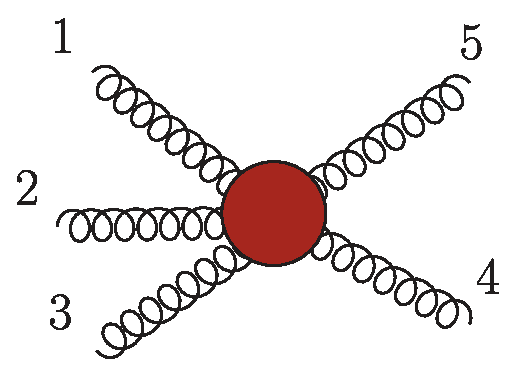
\includegraphics[height=\figureheight]{TreeFull}}} 
    \qquad \xrightarrow[p^2_\xi \to m_\xi^2]{} \quad
    \frac{1}{p^2_\xi - m_\xi^2} \cdot
    \sum_{i\in \text{states}}^{} ~
    \vcenter{\hbox{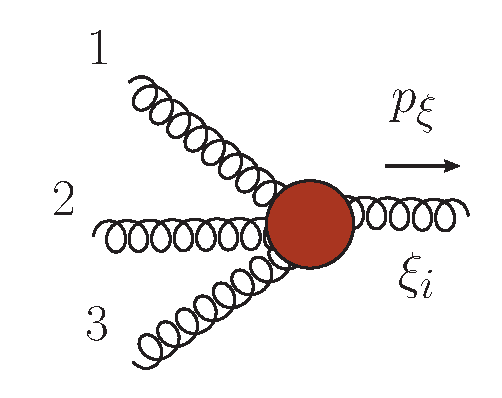
\includegraphics[height=0.9\figureheight]{TreeLeft}}}\cdot
    \vcenter{\hbox{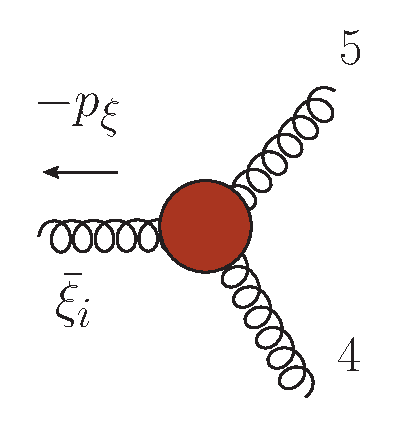
\includegraphics[height=0.9\figureheight]{TreeRight}}}
  \end{equation*}
  \caption{
    An example of factorization due to a physical pole singularity. 
    Here $p_\xi =  p_1 + p_2 + p_3$.
  }
  \label{fig:factorization}
\end{figure}


\todo{Note that in \cref{eq:optical_theorem} there is a phase-space integral present on the right-hand side}

The exact singularity as expected cannot be reached in any physical process.
However if we analytically continue an amplitude to complex external momenta,
it is possible to choose them to hit the pole explicitly
while still satisfying on-shell conditions for external states.


\subsection{On-Shell Recursion}
\label{sec:BCFW}

The universal factorization  property expressed by \cref{eq:factorization_pole} is independent of perturbation theory. 
For tree-level amplitudes however the factorization can be discovered rather straightforwardly by inspection,
although it might be obscured in the expressions found within the standard Feynman-diagrammatic approach.

The factorization of tree amplitudes can be converted into an algorithm to evaluate them.
This is done through the systematic exploration of the amplitude's factorization limits such that
it can be broken down recursively to sums of lower-multiplicity tree amplitudes. 
The building blocks of this recursion are thus on-shell amplitudes.
This idea is known as \emph{Britto-Cachazo-Feng-Witten} (BCFW) recursion \cite{Britto2005c,Britto2005f}.
The on-shell recursion is a very powerful tool for analytical computations, especially 
in theories with supersymmetry \cite{Dixon:2010ik,Drummond:2008cr,Bourjaily:2010wh}.
However for numerical applications and general models the on-shell recursion algorithm
does not offer benefits over off-shell alternatives, both in speed and numerical stability \cite{Duhr:2006iq,Drummond:2008cr,Badger:2012uz},
especially if one is interested in tree amplitudes in arbitrary number of space-time dimensions (see \cref{chap:numunitarity}). 


\subsection{Generalized Cuts}

Unitarity can be turned into a computational method of loop amplitudes as well.
A certain class of one-loop amplitudes, which
can be written as a sum of box, triangle, and bubble scalar integrals,
\begin{equation} \label{eq:cut_constructable_ampl}
  A^{(1)} = \sum_i d_{i}\,\vcenter{\hbox{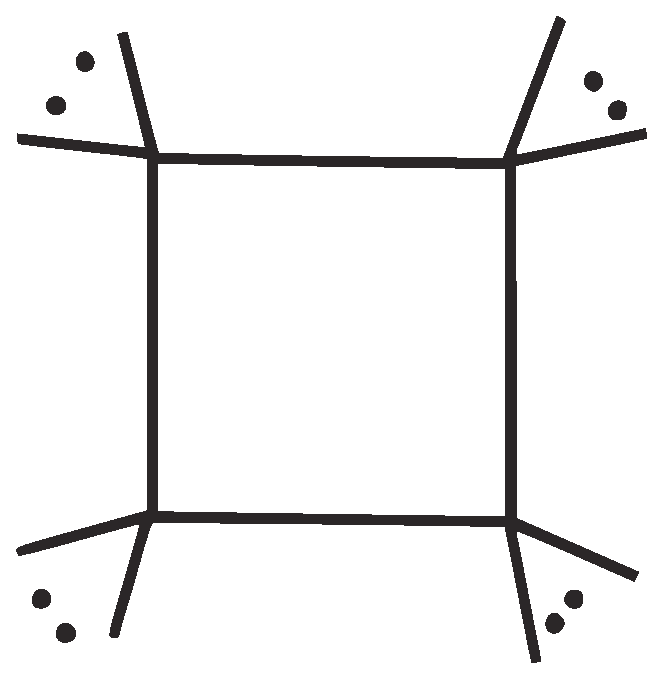
\includegraphics[width=8ex]{boxintegral}}}_i~+~
  \sum_{i}^{} c_{i}\,\vcenter{\hbox{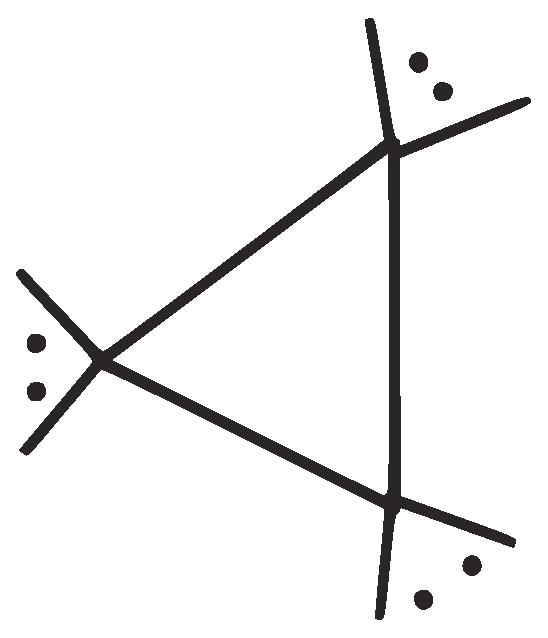
\includegraphics[width=7ex]{triangleint}}}_i~+~
  \sum_i b_{i}\,\vcenter{\hbox{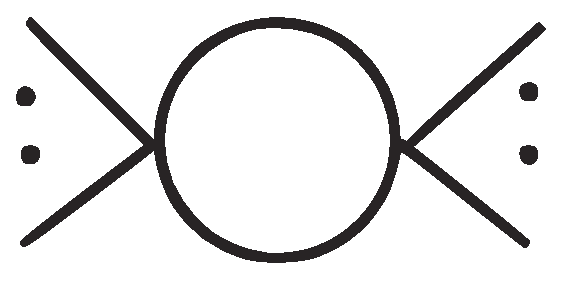
\includegraphics[width=8ex]{bubint}}}_i
\end{equation}
can be obtained entirely from unitarity cuts computed through Cutkosky rules \cite{Bern:1994cg,Bern:1994zx}.
Each integral in \cref{eq:cut_constructable_ampl} has unique discontinuities.
So the discontinuities of the loop amplitude on the left, 
evaluated as phase-space integrals over products of on-shell tree amplitudes as follows from unitarity,
can be matched to those of integrals to obtain equations for the integral coefficients.

However in general \emph{only} unitarity is not enough.

It is possible to generalize application of cuts given by \cref{eq:cut} to
obtain multi-channel discontinuities \cite{Britto:2004nc}.
For example see \cref{fig:quad_cut}.
Note that this kind of cuts are not direct consequences of unitarity of the $\mathcal{S}$-matrix (\cref{eq:unitarity_smatrix}), hence the name \emph{generalized} cuts.

\begin{figure}[ht]
  \centering
  \begin{equation*}
    \vcenter{\hbox{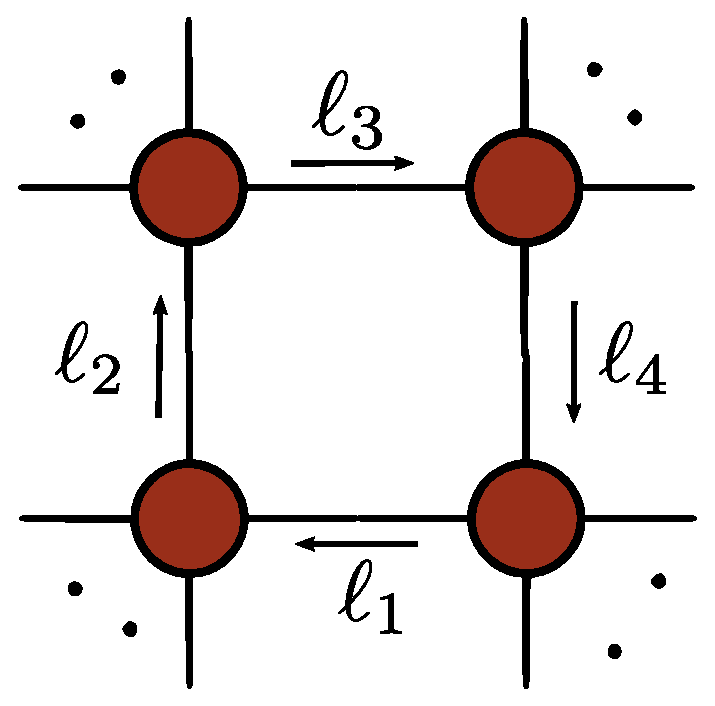
\includegraphics[width=0.2\linewidth]{box}}} \qquad \xrightarrow[i\in\{1\ldots4\}]{\ell_{i}^2-m_i^2\to~0} \qquad
    \vcenter{\hbox{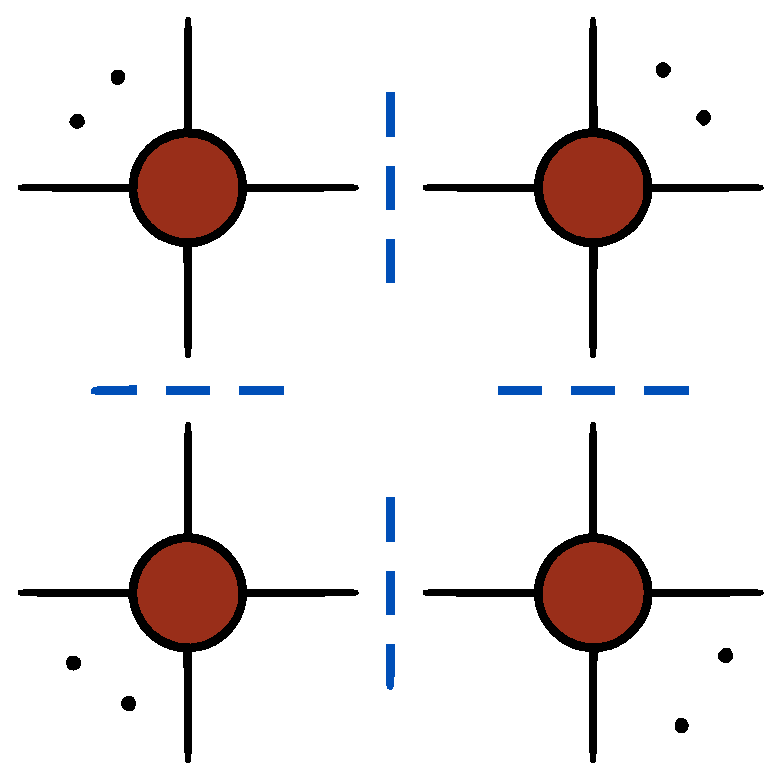
\includegraphics[width=0.2\linewidth]{boxCut}}}
    \quad = \quad \sum_{i}  c_{i} ~ m_{i}(\ell) %+ \sum_{i}  \tilde{c}_{i} \,\tilde{m}_{i}(\ell)
  \end{equation*}
  \caption{
    An example of a generalized cut.
    The loop momentum is chosen such that four propagator are simultaneously put to zero.
    On the left \emph{all} diagrams with the chosen propagators contribute.
    In the factorization limit each corner is a tree amplitude.
    The cut is matched to a basis of loop-momentum polynomials $\{m_i(\ell)\}$ on the right.
  }
  \label{fig:quad_cut}
\end{figure}


As a next step one can use the factorization of amplitudes on the cuts at the \emph{integrand} level  and match
it to a basis of loop-momentum polynomials in numerators (see \cref{fig:quad_cut}),
instead of integral coefficients \cite{Giele:2008ve,Ellis:2007br,Ellis:2008ir,Berger:2008sj}.
This matching procedure is intimately connected to a purely algebraical method of integral reduction known as OPP \cite{Ossola:2006us}.
This method uses the cut conditions \cref{eq:cut} to set some propagators to zero and triangularize linear systems for determining the basis coefficients.
It can be applied individually to each Feynman diagram or a sum thereof, thus having very little to do with factorization and unitarity.
When applied to the full amplitude however, it re

Somewhat confusingly sometimes generalized unitarity methods also refer 

Its flexibility allows for straightforward automation (see e.g.\ \cite{Berger:2008ag,Berger:2008sj,Cullen:2011ac,Mastrolia:2010nb,Ossola:2007ax}).

Most of the ideas mentioned in this section are formulated in the context of one-loop computations.
These give the first real taste of quantum nature of QFT.
Unfortunately, going beyond one-loop, many of the ideas do not generalize straightforwardly,
and require much more sophisticated computational techniques.
The extension of the ideas to multi-loop level have been actively studied in recent years \cite{Ita:2015tya,Abreu:2017idw,Abreu:2017hqn} 

In this thesis we apply the state-of-the-art developments for 

